\section{ラムダ点付近の温度振動解析}
GM冷凍機ではコールドヘッドの瞬時温度がヘリウムの吸入と排出によって振動していることが知られている。本課題においても2段コールドヘッドにおいての温度振動データを取得した。Figure \ref{fig:coldhead_photo}に実験中,センサーとヒータが貼り付けられている位置を示す。
\begin{figure}[h!]
\begin{center}
\includegraphics[width=11cm]{coldhead_photo.png}
\caption{Temperature sensors and heater configuration}
\label{fig:coldhead_photo}
\end{center}
\end{figure}

Figure \ref{fig:temp_osci1}とFigure \ref{fig:temp_osci2}にそれぞれ無負荷条件,1 W/20 mW条件と1 W/0.1 W条件の実測データを示す。

\begin{figure}[h!]
\begin{center}
\includegraphics[width=10cm]{temp_osci_exp.png}
\caption{Experimental data of temperature oscillation on second stage 1}
\label{fig:temp_osci1}
\end{center}
\end{figure}

\begin{figure}[h!]
\begin{center}
\includegraphics[width=10cm]{temp_osci_exp2.png}
\caption{Experimental data of temperature oscillation on second stage 2}
\label{fig:temp_osci2}
\end{center}
\end{figure}

各熱負荷点においての温度振動波形を比較すると,明らかに温度振動の挙動が違うことがわかる。
ここで注目したい挙動の違いは主に:
\begin{enumerate}
\item 温度振動の幅は熱負荷によって変化する。特に2段ステージに加えられている熱負荷が高くなると,振動の幅も大きくなる。20 mWでは振動幅は約40 mKであり,それに対して,0.1 Wを加えた時,振動の幅は350 mKを超えている。
\item 無負荷条件の波形ではピーク2つが現れ,これは負荷ありの条件では見られていない。
\end{enumerate}
この結果について文献\cite{lambda}で詳細な理論分析を行った経緯がある。しかし,著者は把握しているデータが不完全なため,一部計算において簡略化と仮定を用いた。本節は,この論文のアイデアにインスパイアされ,一部詳細検討を加えたものである。最終的には得られた推論に基づいて,到達温度を現状ラムダ点以下までシフトさせる方法を提案する。



\subsection{コールドヘッドの温度挙動分析}
コールドヘッドの温度振動は,ヘリウムの圧縮・膨張によって生じる現象であり,例えば膨張空間内が低圧の時,ロータリバルブの回転によって
膨張空間は高圧ラインと繋がることになり,空間内のヘリウムは高圧になることにつれて,温度も上昇することが想像できるであろう。

一方,実験で測定されたコールドヘッドの温度はヘリウムの挙動だけでなく,コールドヘッドとの熱伝達およびコールドヘッド自身の熱容量も含まれているので
それらの相互関係を分析することが必要になる。Figure \ref{fig:coldhead}に2段膨張空間周囲の構造断面を示す。

\nomenclature{$T_{Cu}$}{Temperature of coldhead (second stage). $(K)$}
\nomenclature{$T_{He}$}{Temperature of helium inside control volume (second stage). $(K)$}
\nomenclature{$m_{Cu}$}{Mass of coldhead (second stage). $(kg)$}
\nomenclature{$c_{Cu}$}{Specific heat of coldhead (second stage). $(J/kg\cdot K)$}
\nomenclature{$\dot Q_a$}{Heat flow from heater to coldhead (+ means the cold head is absorbing heat). $(W)$}
\nomenclature{$\dot Q_x$}{Heat flow from helium inside control volume to coldhead (+ means the cold head is absorbing heat). $(W)$}

\begin{figure}[h!]
\begin{center}
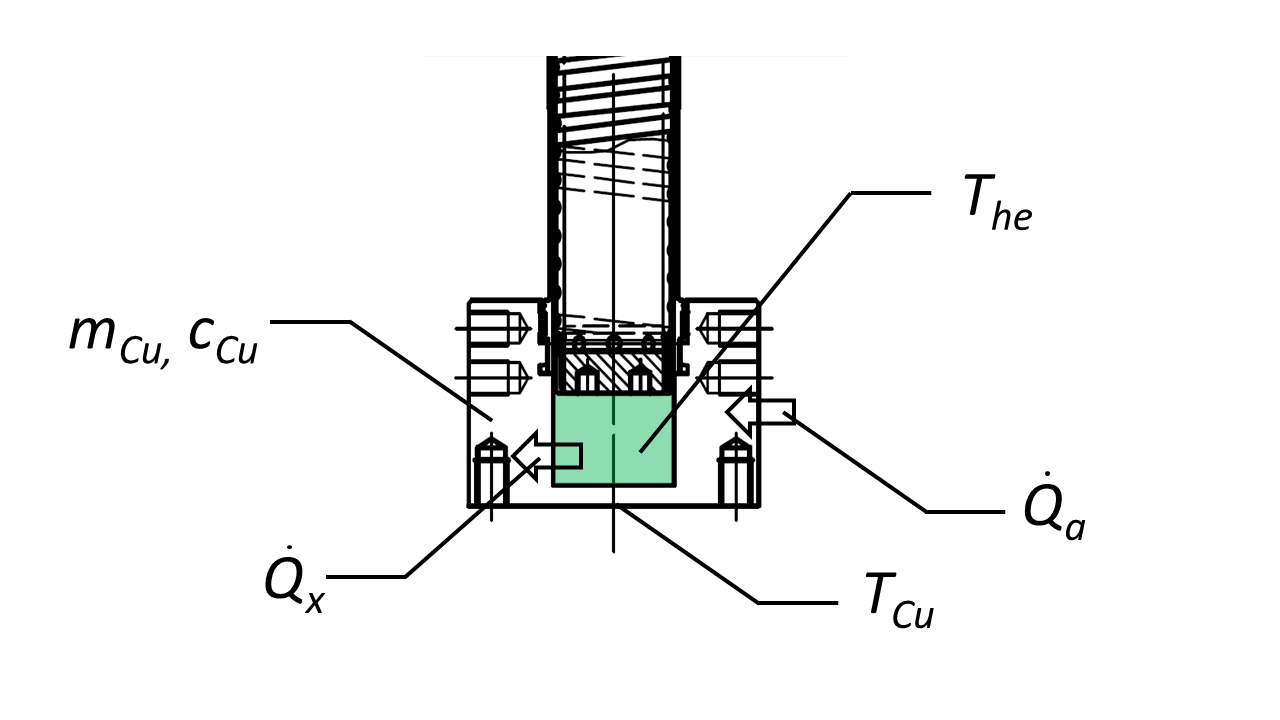
\includegraphics[width=13cm]{coldhead_behavior.png}
\caption{A schematic drawing of second stage coldhead}
\label{fig:coldhead}
\end{center}
\end{figure}

ここの$\dot Q_a$は外部ヒータ及び熱伝導による侵入熱がコールドヘッド(銅ブロック)に与える熱流$(W)$,$\dot Q_x$は膨張空間内のヘリウムがコールドヘッドに与える熱流$(W)$を意味する。またコールドヘッドが吸熱する場合を正とし,逆に銅ブロックが熱を放出する場合は負とする。コールドヘッドを分析対象とし
エネルギー保存則を適用するとヘリウム温度とコールドヘッド温度は以下の式で関連付けられることがわかる:

\begin{equation}
\dot Q_a + \dot Q_x = m_{Cu} c_{Cu} \frac{\partial T_{Cu}}{\partial t}
\end{equation}
\begin{equation}
\dot Q_x = h_xA_x(T_{He} - T_{Cu})
\end{equation}

\nomenclature{$h_x$}{Heat transfer coefficient between Helium and cold head (in second stage expansion room). $(W/m^2\cdot K)$}
\nomenclature{$A_x$}{Heat transfer area (inside second stage expansion room).}

ここの熱伝達率$h_x$と熱交換面積$A_x$は時間とともに変化する以外多くの条件に依存しているので簡易計算では正確に与えることは困難。
一方,これらを定数だと仮定すれば物理現象が理解しやすくなるのでここではこれらを定数だとする。上記の式から温度変数を分離するよう
整理すると:

\begin{equation}
\dot Q_a +h_xA_x(T_{He} - T_{Cu}) = m_{Cu} c_{Cu} \frac{\partial T_{Cu}}{\partial t}
\end{equation}
\begin{equation}
T_{He} = T_{Cu} + \frac{m_{Cu} c_{Cu}}{h_x A_x} \cdot \frac{\partial T_{Cu}}{\partial t} - \frac{\dot Q_a}{h_x A_x}
\label{eqn:coldhead-helium}
\end{equation}

式\ref{eqn:coldhead-helium}は,制御工学の視点から見ると,コールドヘッド表面の温度$T_{Cu}$はヘリウム温度$T_{He}$に対して1次遅れ応答になっている。
すなわち式\ref{eqn:coldhead-helium}を,時間を自変数としてラプラス変換を施すと下の形になり:

\begin{equation}
\mathcal{L} \{T_{He} + \frac{\dot Q_a}{h_x A_x}\} = \mathcal{L} \{ T_{Cu}\} + \frac{m_{Cu} c_{Cu}}{h_x A_x} \cdot \mathcal{L} \{ T_{Cu}\} \cdot s
\label{eqn:coldhead-helium_laplace}
\end{equation}

\nomenclature{$\mathcal{L}$}{Laplace transformation symbol.}
\nomenclature{$s$}{Complex number frequency used in Laplace transformation.}

これに基づいて解析解,あるいはフーリエ変換を使うことで周波数領域の応答を求めることもできるが,今回は測定された$T_{Cu}$からヘリウム温度$T_{He}$を逆算したいので,式\ref{eqn:coldhead-helium}に戻って離散化方法で結果を算出することにする。

ここで式\ref{eqn:coldhead-helium}に含まれている温度以外の変数も定めないといけないが,これらの量の正確な値を測定するのは困難。ある程度の簡略化をするため,熱伝達率を表す$(h_x A_x)$を定数とする。無負荷の場合,コールドヘッドに入る熱$\dot Q_a$は熱伝導による熱侵入のみを持ち,この量は約40-60 mWだと試算される。また銅ブロックの熱容量については,銅の物性及び実際の体積から計算する。
5 K以下の銅の物性は文献\cite{copper_cp}から得られ,下記の式で計算できる:

\begin{equation}
c_{Cu} = 11.17T + 0.0757T^3 \mu J/gK
\label{eqn:copper_cp}
\end{equation}

現設計のコールドヘッドは約$50cm^3$であり,この式と合わせて2.1 K付近での熱容量は約$9.2mJ/K$になる。式\ref{eqn:coldhead-helium}において入熱$\dot Q_a$と同じオーダーだがせいぜいそれの1/4程度である。

クリアランス熱交換器の熱伝達率$h_x$を概算(あくまでもオーダーの概算にすぎない,正確な値ではない)するため,平板間の強制対流熱伝達率関連式を使用する:

\begin{equation}
Nu = 0.664Re^{1/2}Pr^{1/3}
\label{eqn:heatx_corr}
\end{equation}

詳細説明は省略するがレーノルズ数と熱伝達率を算出するプロセスを記載しておく。

\begin{gather*}
V_{exp}=\frac{1}{4} \pi 18^2 \cdot 12 \approx 3.05 \times 10^3 (mm^3) = 3.05 \times 10^{-6} (m^3) \\
\Delta m = \rho (2.05 MPa, 2.1 K) \cdot V_{exp} =172.1(kg/m^3) \cdot 3.05 \time 10^{-6} (m^3) \approx 5.25 \times 10^{-4} (kg) \\
\dot M = \frac{\Delta m}{\Delta t_{charge}} = 1.05\times10^{-3} (kg/s) \\
Clearance\; size:\;about\; 0.5mm\\
U_{ave} = \frac{\dot M}{\rho(2.05 Mpa,2.1 K)\cdot A_{open}} = \frac{1.05\times10^{-3}}{172.1 \cdot  0.5\cdot \pi \cdot 18\times 10^{-6}} \approx 0.216 (m/s)\\
Characteristic\; length\; = 2\cdot 0.5 = 1mm\\
Re_{ave} = \frac{\rho(2.05 MPa,2.1 K) U_{ave} D_h}{\mu(2.05 MPa, 3.6 K)} = \frac{172.1 \cdot 0.216 \cdot 1.0\times 10^{-3}}{7.01\times10^{-6}} \approx 5300 \\
Nu_{ave} = 0.664 \cdot Re_{ave}^{1/2}Pr(2.05 MPa,3.6 K)^{1/3} \approx 40.8\\
h_x = Nu_{ave}\cdot D_h / \lambda(2.05 MPa,3.6 K) \approx 1.7 (W/m^2\cdot K)\\
h_x \cdot A_x = 1.7\cdot (\pi \cdot 18 \cdot 10 \times 10^{-6}) \approx 0.97(mW/K)\\
\end{gather*}

以上計算式の一部の物性値(例えば2.1 Kにおけるヘリウムの粘性)はNISTデータベースに存在しないので,直近のデータを使うことにした。もしこの結果が正しいとすると,ヘリウム温度$T_{He}$は銅ブロック温度よりも遥かに低くなっていると計算される。しかし銅ブロック温度でもすでに2 K台になっているので,ヘリウム温度は絶対0 Kに近づいているとは考えにくい。従って以上の計算は信頼できないと考えられる。実際熱交換係数$h_x$が上記計算結果を上回る事が可能な理由としては,ヘリウムの粘性が非常に0に近づいていることと,ヘリウムの一部が超流体に転移していることがあげられる。いずれも超流体付近のヘリウム熱伝達特性と関係し,正確に算出することは本稿の範疇を超えている。また,熱負荷フランジとヘリウムの熱交換はクリアランスだけでなく,底面部分も寄与していると考えられるので,本来は少なくとも2次元流れ場の計算が必要だが,本稿では時間の関係で実施できておらず,これらについて将来の課題にする。

故に,物性データが不足している中上記の$h_x$を確定することは困難であり,ここでは,ラムダ点付近においてヘリウムの粘性が非常に0に近づいていると仮定し,$h_x$にいくつかの値を与え,計算結果を示すことにする。

\begin{figure}[h!]
\begin{center}
\includegraphics[width=12cm]{1w20mw_cal.png}
\caption{Experimental data of temperature oscillation compared with predicted helium temperature}
\label{fig:1w20mw_cal}
\end{center}
\end{figure}

Figure \ref{fig:1w20mw_cal}から,先ず温度プロファイルの形状が非常に類似していることが判明された。これの理由は,先の計算で示したとおり,銅ブロック自身の熱容量が非常に小さいことにあると考えられる。また,熱交換率$h_x$の増大とともに,ヘリウム温度は測定温度プロファイルに近づくことも判明した。以降の分析では,ヘリウム温度が実測された銅ブロック表面の温度とほぼ同じであると仮定し,分析を行っていく。

\subsection{温度振動と圧力波形のカップリング}

前節までは,実験で測定された銅ブロックの表面温度と実際膨張空間内のヘリウム温度の関係について分析した。膨張空間内のヘリウム温度振動は,圧力の変動に起因されているので,ここからは,この二つの関係について分析する。

前節の分析で判明されたよう,熱侵入$Q_a$は温度波形の上下スライドのみをもたらし,温度波形の形状には影響が少ない。そこで,この項を無視し,即ちヘリウムの膨張を断熱であると仮定し,波形の再現性を検証する。断熱膨張工程において,ヘリウムのエントロピーは一定であるため,温度は圧力のみで一意に定まる。

Figure \ref{fig:temp_osci1}から,圧力ピーク時の温度は約2.3 Kとなっていることから,先ずその時のヘリウムエントロピーを調べ,Figure \ref{fig:nist_entropy}にNISTデータベースから得られた,エントロピー$s_{he}$=1556 $J/kg\cdot K$時のヘリウム物性データを示す。

\nomenclature{$s_{he}$}{Specific entropy (entropy of unit mass) of helium. $(J/kg\cdot K)$}

\begin{figure}[h!]
\begin{center}
\includegraphics[width=13cm]{nist_entropy.png}
\caption{Helium property data from NIST database}
\label{fig:nist_entropy}
\end{center}
\end{figure}

同様に,無負荷時のヘリウム物性データも,Figure \ref{fig:temp_osci1}のピーク時の温度からエントロピー値を逆算することで獲得することができる。これらのデータを,シミュレーションで得られた膨張空間内の圧力振動データに適用し,もし実測データと一致していれば,上記の分析や仮定は適切であることが言えるであろう。Figure \ref{fig:entropy1556}とFigure \ref{fig:entropy1400}にこの方法で得られた圧力と温度の関係を示す。1 W/20 mWの場合とは異なり,Figure \ref{fig:entropy1400}で示されている無負荷時の線は,ヘリウムがラムダ点に近づいているため,極小点が現れ,それより左の領域において圧力の減少とともに温度は逆に上昇する。

\begin{figure}[h]
\begin{center}
\includegraphics[width=11cm]{entropy1556.png}
\caption{Temperature and pressure relation when entropy = 1556 $J/kg\cdot K$}
\label{fig:entropy1556}
\end{center}
\end{figure}

\begin{figure}[h]
\begin{center}
\includegraphics[width=11cm]{entropy1400.png}
\caption{Temperature and pressure relation when entropy = 1442 $J/kg\cdot K$}
\label{fig:entropy1400}
\end{center}
\end{figure}

Figure \ref{fig:temp_osci_cal}は計算した温度振動波形と実際実測した温度波形の比較を示している。この結果から,温度振動はヘリウムの断熱膨張による物性変化に支配されていることが判明した。


\begin{figure}[h]
\begin{center}
\includegraphics[width=13cm]{temp_osci_cal.png}
\caption{Calculated temperature oscillation compared with experiment data}
\label{fig:temp_osci_cal}
\end{center}
\end{figure}


\subsection{2 K以下を達成する方策}

前節Figure \ref{fig:entropy1400}から,ヘリウムが断熱膨張をする際,減圧することのみでは極小点以下に到達するのは不可能であることが判明した。一方,この極小点(実際はヘリウムの体積膨張係数の正負逆転点)は,圧力の増加とともに下がる性質がある。

\begin{figure}[h]
\begin{center}
\includegraphics[width=13cm]{alpha_slide.png}
\caption{Minimum point shifting on a isentropic line of Helium (Entropy unit: $J/kg\cdot K$)}
\label{fig:alpha_slide}
\end{center}
\end{figure}

Figure \ref{fig:alpha_slide}はヘリウムの等エントロピー線を、圧力、温度軸でプロットしたものであり,これらの等エントロピー線の形状から分かるよう,系の圧力が1 MPaと2 MPaの間にある時,温度の極小点は2.0 K付近にあることに対し,圧力を3 MPaまで上げることで,2.0 K以下となる。即ち,従来設計ではこの極小点に制限され,2.0 K以下まで到達することは不可能だが,全体圧力を3 MPa以上まで上昇させることで2.0 K以下を到達する可能性が現れてくる。

但し,現時点で試作機の強度設計や,シール設計は3 MPaでの運転を想定していないため,試験で検証することは困難。これについては,将来筐体の強度設計を見直し,リニア圧縮機と組み合わせで実施する予定とする。

\begin{figure}
\centering
\begin{python}
#
from pyx import *
import time
print "Hello \LaTeX! from Python !!"
print "This version is compiled at: "+time.ctime()
g = graph.graphxy(width = 11, x=graph.axis.linear(min=-15, max=15),y=graph.axis.linear(min=-0.25, max=1.5), key=graph.key.key(pos="tr", dist=0.1))
g.plot([graph.data.function("y(x)=sin(x)/x", title="This graph"),
graph.data.function("y(x)=0.7*sin(x)/x", title="is created to"),
graph.data.function("y(x)=0.6*sin(x)/x", title="occupy"),
graph.data.function("y(x)=0.5*sin(x)/x", title="the extra white space ...")], 
[graph.style.line([color.gradient.Rainbow])])
g.writePDFfile("function")
print r'\includegraphics{function}'
\end{python}
\caption*{$y(x)=\frac{\sin(x)}{x}$ plotted by PyX from embedded Python script}
\end{figure}

